\documentclass[a4paper,12pt]{article}
\usepackage[a4paper, margin=2cm]{geometry}
\usepackage[utf8]{inputenc}
\usepackage{amsmath, amssymb} % Packages pour les maths
\usepackage[T1]{fontenc}
\usepackage{graphicx} 
\usepackage{caption}
\usepackage{hyperref}
\usepackage{setspace} % Espacement des lignes
\usepackage{tikz}
\usepackage{soul}
\usepackage[inkscapelatex=false]{svg}


\usepackage{titlesec}
\usepackage{hyperref}
\renewcommand{\contentsname}{Table des matières}
\usepackage[color'links=true, linkcolor=blue, urlcolor=blue, citecolor=blue]{hyperref}
\titleformat*{\section}{\LARGE\bfseries}
\titleformat*{\subsection}{\Large\bfseries}
\titleformat*{\subsubsection}{\normalsize\bfseries}
\titleformat{\part}[display]
  {\normalfont\Huge\bfseries}{}{0pt}{}
\begin{document}
\begin{titlepage}
    \centering
    % Logo en haut, optionnel
    % \includegraphics[width=0.25\textwidth]{chemin/vers/logo.png}\par\vspace{1cm}

    \vspace*{2cm}
    
    {\LARGE \textsc{CapECL}}\\[1.5cm] % Titre secondaire
    
    {\Huge \bfseries Document de Synthèse}\\[0.5cm]
    {\Large \itshape}\\[2cm] % Sous-titre stylisé

    \rule{\textwidth}{0.4pt}\\[0.4cm]
    {\large Projet Climat}\\[0.2cm]
    {\large  2024–2025}\\
    \rule{\textwidth}{0.4pt}\\[2cm]
    
    \vfill
    
    {\large Réalisé par :}\\
    {\large  Les Carcajous Callipyges}\\[0.5cm]

    {\large }\\
    {\large Taha Thaïs Candice Léna Chloé Pierre-Louis Camille Romain Elise Melvin Elsa}\\[1cm]

    \vfill

\end{titlepage}

\tableofcontents
\newpage
\addcontentsline{toc}{section}{Introduction}
{\LARGE \textbf{Introduction\\}}


Ce projet a pour but de modéliser de manière dynamique l'évolution de la température terrestre au cours du temps et de l'espace. L'idée est simple : partir d’une vision très simplifiée de notre planète, puis ajouter progressivement des éléments pour se rapprocher d’une description plus réaliste.

Quatre modèles ont été développés, chacun apportant une amélioration supplémentaire : 

\begin{itemize}
    \item \hyperref[sec:modèle 1]{\textbf{Modèle 1}} : La Terre est vue comme une simple sphère (ou coquille) d’eau dans le vide, sans atmosphère ni apport solaire. Elle perd sa chaleur uniquement par rayonnement.
    
    \item \hyperref[sec:modèle 2]{\textbf{Modèle 2}} : Une atmosphère est introduite. Elle permet à la Terre d’échanger de la chaleur avec l’extérieur par conduction thermique.
    
    \item \hyperref[sec:modèle 3]{\textbf{Modèle 3}} : L’intérieur de la coquille n’est plus vide. On considère donc  les échanges thermiques internes entre le centre de la Terre et sa surface.
    
    \item \hyperref[sec:modèle 4]{\textbf{Modèle 4}} : C’est le modèle le plus complet. Il prend en compte la géographie réelle (continents, océans), l’albédo du sol et des nuages, la chaleur latente, les capacités thermiques variables selon les régions, et des données climatiques réelles.
\end{itemize}

Les schémas ci-dessous montrent l’évolution des modèles :



   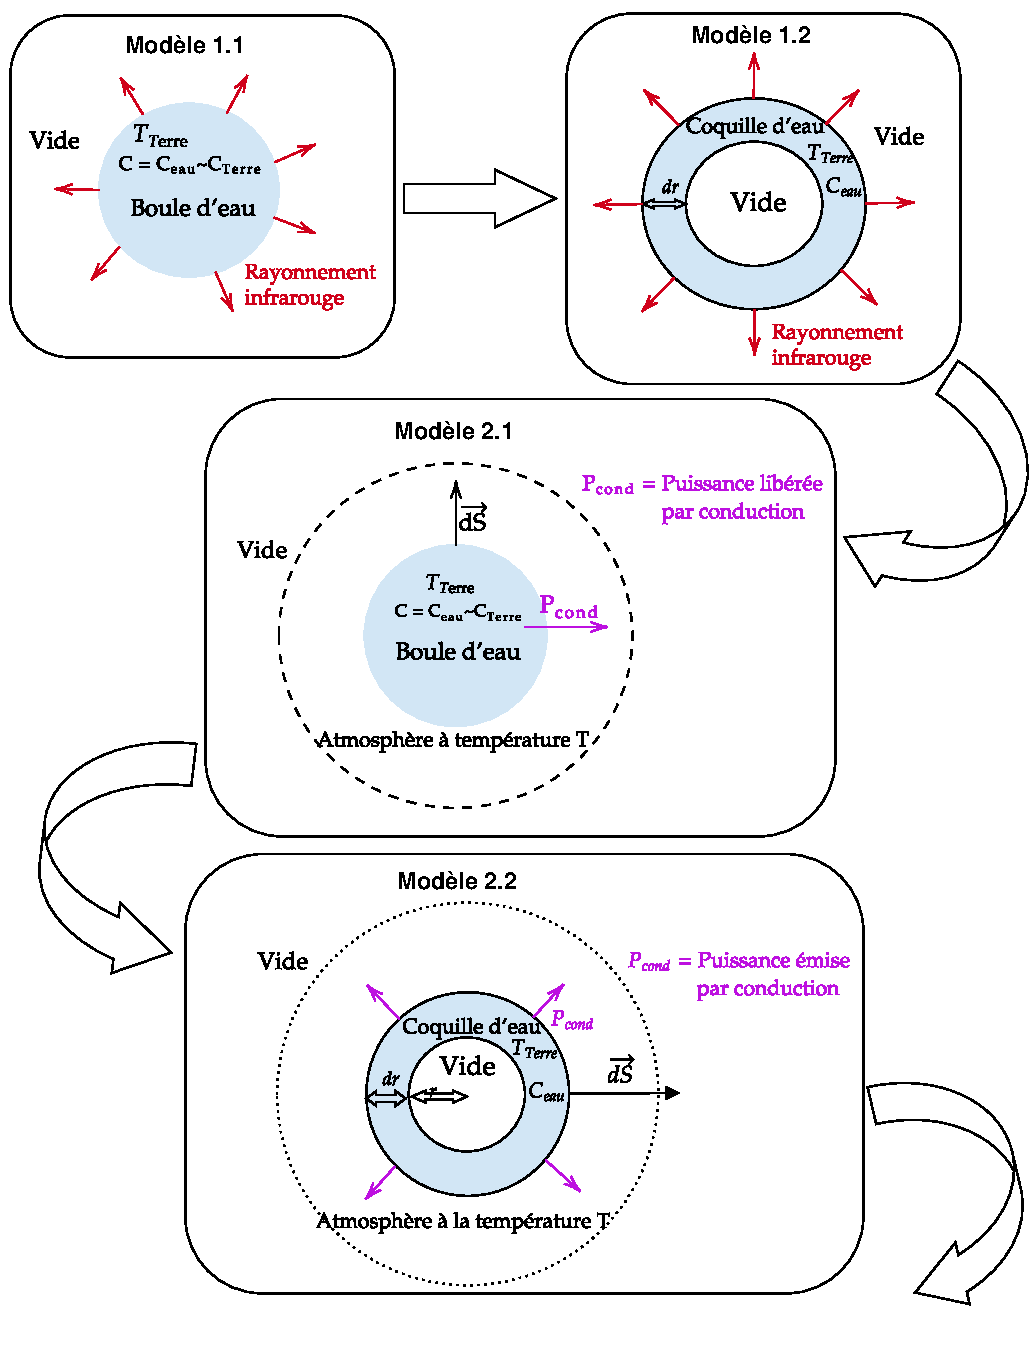
\includegraphics[width=1\textwidth, angle=0]{evolution_projet_1.pdf}


\\
\\
\begin{center}
   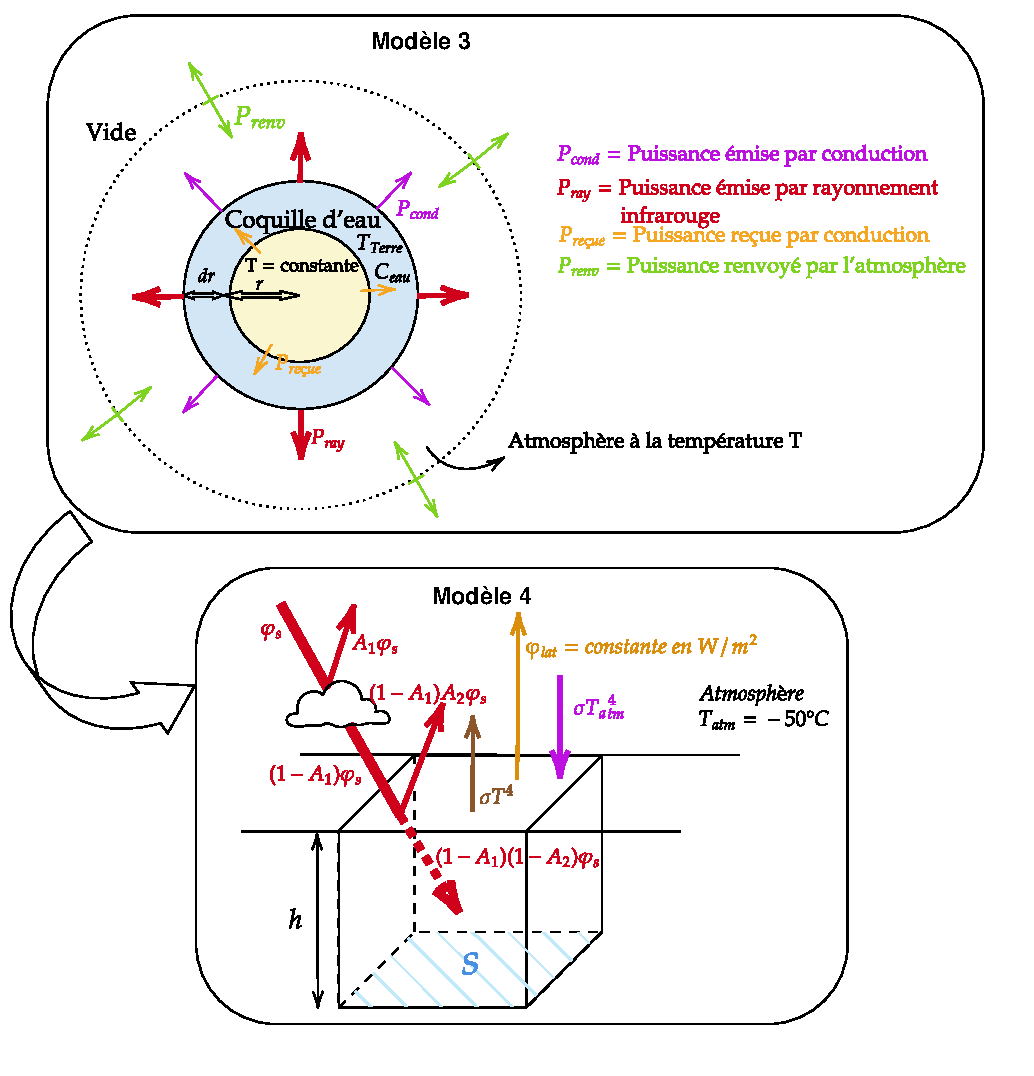
\includegraphics[width=1\textwidth, angle=0]{evolution_projet_2.pdf}
\end{center}

\newpage
  
\section{Modèle 1: }
\label{sec:modèle 1}
\subsection{Boule d’eau rayonnante dans le vide}
\addcontentsline{toc}{subsubsection}{Hypothèses} 
\textbf{Hypothèses}

\begin{itemize}
    \item Terre assimilée à une \textbf{boule d'eau}, de température
    \(T_{\text{Terre}}\) telle que \(T_{\text{Terre}}\)> \(T_{\text{ext}}\)
    \item  Sans atmosphère (dans le vide)
    \item  Sans puissance solaire reçue  
    \item \(c_{m}= c_{\text{m,eau}} \sim c_{\text{m,Terre}}\) 
    \item $T(t=0) = T_i$ \ \ \
$T(t \to +\infty) = T_0$
   
\end{itemize}
$\rightarrow$ la terre perd de la température par \textbf{rayonnement}
\\ 

\addcontentsline{toc}{subsubsection}{Schéma}
\textbf{Schéma}
\\
\noindent\textcolor{gray}{\rule{\linewidth}{0.4pt}}

    
\begin{center}
  \input{modele1/figures/Schéma mathcha modèle 1.1.txt}
\end{center}



\noindent\textcolor{gray}{\rule{\linewidth}{0.4pt}} 

\vspace{1cm}

\addcontentsline{toc}{subsubsection}{Equation}
\textbf{Équation}

\begin{align*}
P &= \sigma T^4 \cdot S \\
C \, \frac{dT}{dt} &= - \sigma T^4 \cdot S \\
\frac{dT}{dt} &= \boxed{ - \frac{4 \pi R_T^2 \sigma T^4}{C} }
\end{align*}

Avec 
\(S= 4\pi r^2\)
\ \ \ \
\(\sigma=5{,}67 \cdot 10^{-8} \, \mathrm{W \cdot m^{-2} \cdot K^{-4}}\)

\vspace{0.5cm} 
\addcontentsline{toc}{subsubsection}{Solution}
\textbf{Solution} 
\\

\boxed{
T(t) = \left( \frac{C}{C/T_i^3 + 12\pi R^2 \sigma t} \right)^{1/3} 
= \frac{T_i}{\left(1 + 3k T_i^3 t \right)^{1/3}}}
\\
\vspace{0,2cm}
\\
avec \(k=\frac{4\pi R_T^2 \sigma}{C}\)  
et \(C=c_{\text{m eau}}\times m=4{,}60 \cdot 10^{27} \, \mathrm{J \cdot K^{-1}}\)

\vspace{1cm} 
\addcontentsline{toc}{subsubsection}{Modélisation graphique}
\textbf{Modélisation graphique} 

\begin{center}
  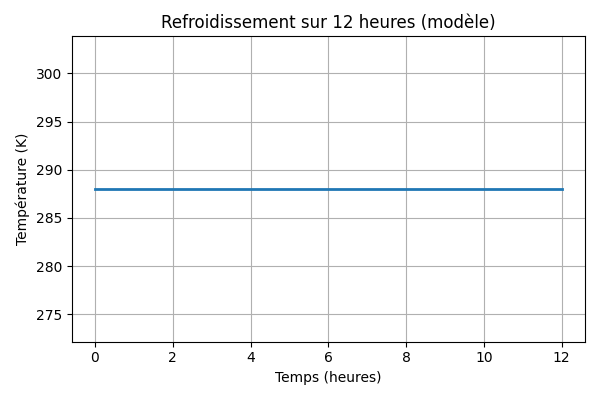
\includegraphics[width=0.8\linewidth]{../modele1/figures/modele1.png}
\end{center}

    
    

\subsection{Coquille d’eau rayonnante (intérieur vide) }
\addcontentsline{toc}{subsubsection}{Hypothèses}
\textbf{Hypothèses}
\begin{itemize}
    \item On garde les hypothèses précédentes, excepté le système: la Terre est assimilée à une \textbf{coquille d'eau}, d'épaisseur dr, qui a un \textbf{intérieur vide}
    
\end{itemize}
$\rightarrow$ il faut donc recalculer la capacité thermique 

\vspace{0.5cm} 
\addcontentsline{toc}{subsubsection}{Schéma}
\textbf{Schéma}


\noindent\textcolor{gray}{\rule{\linewidth}{0.4pt}}

    
\begin{center}
  \input{modele1/figures/Schéma modèle 1.2 coquille.txt}
\end{center}



\noindent\textcolor{gray}{\rule{\linewidth}{0.4pt}} 

\vspace{1cm}


\addcontentsline{toc}{subsubsection}{Calcul capacité thermique}
\textbf{Calcul capacité thermique}

\begin{align*}
m &= \rho_{\text{eau}} \left( \frac{4}{3} \pi (R_T + dr)^3 - \frac{4}{3} \pi R_T^3 \right) \\
&\overset{DL}{\approx} \rho_{\text{eau}} \cdot 4\pi R_T^2 \cdot dr \\
\\
C &= c_{\text{m,eau}} \cdot \rho_{\text{eau}} \cdot 4\pi R_T^2 \cdot dr \\
&= 4{,}31 \cdot 10^{20} \ \text{J} \cdot \text{K}^{-1} \\
\\
k &= \boxed{\frac{\sigma }{c_{\text{eau}} \cdot \rho_{\text{eau}} \cdot dr}}
\end{align*}
\vspace{0.5cm}
\subsubsection*{Modélisation graphique}   
\begin{center}
  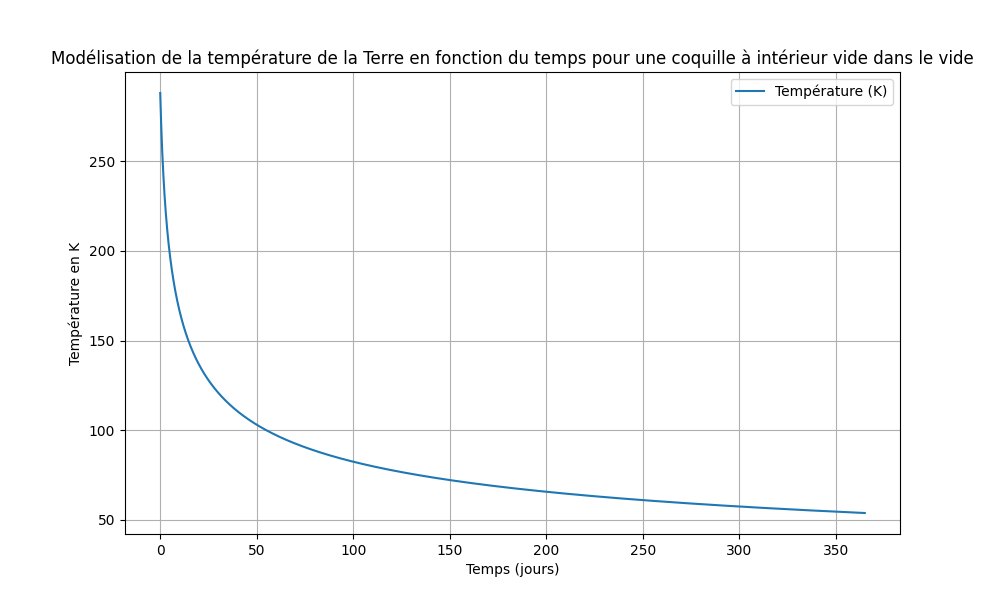
\includegraphics[width=0.8\linewidth]{../modele1/figures/modele1_coquille.png} 
\end{center}



\subsection{Critique du modèle}

\begin{itemize}
    \item Pas d’atmosphère, pas de rayonnement thermique reçu du Soleil, uniquement un transfert thermique émis par rayonnement.
    \item La Terre est assimilée à de l’eau.
    \item Température de la Terre subjective.
    \item Température du vide subjective.
    \item Épaisseur de la coquille arbitraire.
    \item On a supposé l'intérieur de la coquille vide, or cela implique un rayonnement à la fois vers l'intérieur et vers l'extérieur de la coquille.
\end{itemize}  

\newpage
\section{Modèle 2 : Terre avec atmosphère conductrice}
\label{sec:modèle 2}
\subsection{Boule d’eau avec atmosphère conductrice }
\addcontentsline{toc}{subsubsection}{Hypothèses}
\textbf{Hypothèses}
\begin{itemize}
    \item Terre assimilée à une \textbf{boule d'eau}, de température \(T_{\text{Terre}}\) 
    \item  \textbf{Atmosphère} avec une température uniforme T 
    \item  Sans puissance solaire reçue  
    \item  Sans convection  
    \item \(c_m=c_{\text{m,Terre}}\sim c_{\text{m,eau}}\) 
    \item $T(t=0) = T_i$ \ \ \
$T(t \to +\infty) = T_0$
    \item La Terre ne rayonne pas
   
\end{itemize}
\vspace{0.5cm}
\subsubsection*{Schéma :} 
\noindent\textcolor{gray}{\rule{\linewidth}{0.4pt}}

\begin{center}
  \input{modele2/figures/Schéma mathcha modèle 2.1.txt}
\end{center}
\noindent\textcolor{gray}{\rule{\linewidth}{0.4pt}}
\vspace{0.5cm}

\addcontentsline{toc}{subsubsection}{Équations de transfert thermique}
\textbf{Équations de transfert thermique}

On applique le premier principe au système \{ boule d'eau  \}

\begin{align*}
\delta Q = C\, dT &= -P_{\text{th,cond}} \cdot dt \\
\Rightarrow -\int \int \vec{j_{\text{th,cond}}}\, \vec{dS}\,dt &= C\, dT \\
\Rightarrow -\int_{\theta=0}^\pi \int_{\phi=0}^{2\pi} h(T - T_0) \vec{e_{\text{r}}}\cdot r^2 \sin\theta\, d\theta\, d\varphi \vec{e_{\text{r}}}\, dt &= C\, dT \\
\Rightarrow -h(T - T_0) \cdot 4\pi\, dt &= C\, dT \\
\Rightarrow -T + T_0 &= \frac{C}{h 4\pi} \frac{dT}{dt} \\
\Rightarrow \frac{dT}{dt} &= -\frac{4\pi h}{C}(T - T_0)
\end{align*}


\vspace{0.5cm}

\addcontentsline{toc}{subsubsection}{Solution}
\textbf{Solution} 
$T(t) = T_0 + (T_i - T_0)e^{-kt}$ \quad avec $k = \frac{4\pi h}{C}$
\\
\bigskip

\addcontentsline{toc}{subsubsection}{Modélisation graphique}
\textbf{Modélisation graphique}
\begin{center}
  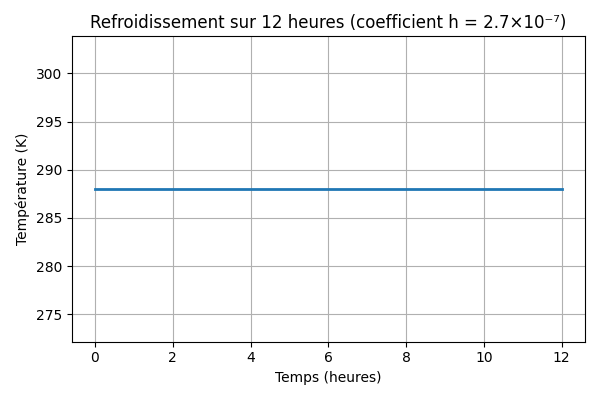
\includegraphics[width=0.8\linewidth]{../modele2/figures/modele2.png}
\end{center}
    
\vspace{1cm}
\subsection{Coquille d’eau avec atmosphère conductrice }
\addcontentsline{toc}{subsubsection}{Hypothèses}
\begin{itemize}
    \item On garde les hypothèses précédentes, en ajoutant l'\textbf{atmosphère} \end{itemize}
\vspace{1cm}
\addcontentsline{toc}{subsubsection}{Schéma}
\textbf{Schéma}
\\
\noindent\textcolor{gray}{\rule{\linewidth}{0.4pt}}

    
\begin{center}
  \input{modele2/figures/Schéma modèle 2.2 coquille.txt}
\end{center}
\noindent\textcolor{gray}{\rule{\linewidth}{0.4pt}}
\vspace{0.5cm}
\addcontentsline{toc}{subsubsection}{Modélisation graphique}
\textbf{Modélisation graphique}
\begin{center}
  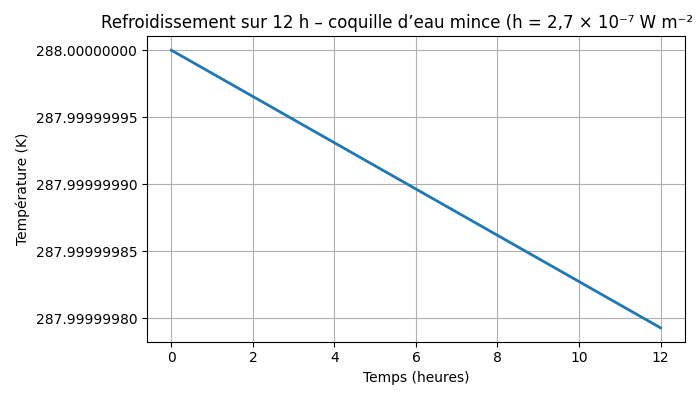
\includegraphics[width=0.8\linewidth]{../modele2/figures/modele2_coquille.png}
\end{center}
        


\subsection{Critique du modèle}

\begin{itemize}
    \item Température de la Terre subjective.
    \item Épaisseur de la coquille.
    \item Prise en compte de l’atmosphère donc utilisation de la loi de Newton :
    \begin{itemize}
        \item problème de définition de la couche limite : convection non prise en compte
    \end{itemize}
    \item Dans les codes {\href{https://github.com/pierrelouis-cmrt/CREPES/blob/main/modele2/codes%20python/modele2_coquille.py}{modele2\_coquille.py}} et {\href{https://github.com/pierrelouis-cmrt/CREPES/blob/main/modele2/codes%20python/modele2_boule.py}{modele2\_boule.py}}, on a posé $h = \lambda_{\text{air}} / \delta$ avec $\lambda_{\text{air}} = 0{,}027 \, \mathrm{W/(K \cdot m)}$.
    \begin{itemize}
        \item $\delta = 100\, \mathrm{km}$ : longueur de la couche limite surestimée
        
    \end{itemize}
    \item Problème de définition de $T_0$ :
    \begin{itemize}
        \item température au-delà de la thermosphère (or on a posé $T_0 = 273\, \mathrm{K}$ dans nos codes Python).
    \end{itemize}
\end{itemize}

\newpage
\section{Modèle 3 : Coquille d’eau avec intérieur conducteur }
\label{sec:modèle 3}
{\Large \textbf{Conduction interne + rayonnement externe}}
\addcontentsline{toc}{subsubsection}{Hypothèses}

\vspace{0.5cm}
\textbf{Hypothèses}
\begin{itemize}
    \item Terre assimilée à une \textbf{coquille d'eau} avec intérieur \textbf{non vide}
    \item  conduction entre centre de la terre et croûte (\(P_r\))
    \item  conduction entre croûte et air (\(P_{th,cond}\))
    \item  rayonnement de la croûte (\(P_{th,ray}\))
    \item On néglige le rayonnement de l'atmosphère
    \item $T(t=0) = T_i$ \ \ \
$T(t \to +\infty) = T_0$
     
\end{itemize}


\addcontentsline{toc}{subsubsection}{Schéma}

\textbf{Schéma}
\\
\noindent\textcolor{gray}{\rule{\linewidth}{0.4pt}}

    
\begin{center}
  \input{modele3/figures/Schéma modèle 3 coquille.txt}
\end{center}
\noindent\textcolor{gray}{\rule{\linewidth}{0.4pt}}
\vspace{0.5cm}
\addcontentsline{toc}{subsubsection}{Équations de transfert thermique}

\textbf{Équations de transfert thermique}

On applique le premier principe au système \{ coquille non vide  \}
\[
(-P_{\mathrm{th,cond}} - P_{\mathrm{th,ray}} + P_r)\,dt = C\,dT.
\]

\[
-\,h\bigl[T(r+dr)-T_0\bigr]\;4\pi
\;-\;4\pi\,\cdot (r+dr)^2\,\sigma\,T^4(r+dr)
\;-\;4\pi\,r^2\,\lambda\,\frac{\partial T}{\partial r}(r)
\;=\;C\,\frac{dT}{dt}.
\]

\medskip

Or au \(1^{er}\) ordre en \(dr\), \(r+dr\approx r\) :
\\

\boxed{
-4\pi\,h\bigl(T(r)-T_0\bigr)
\;-\;4\pi\,r^2\,\sigma\,T(r)^4
\;-\;4\pi\,r^2\,\lambda\,\frac{\partial T}{\partial r}(r)
\;=\;C\,\frac{dT}{dt}}


\medskip

Avec
\[
P_{r}
= \iint\vec j_{\mathrm{thr}}\cdot d\vec S
= \iint -\lambda\,\vec{ \nabla } T\cdot d\vec S
= -\lambda
  \int_{0}^{\pi}\!\!\int_{0}^{2\pi}
    \frac{\partial T}{\partial r}\,\vec e_{r}\,
    r^2\sin\theta\;d\theta\,d\varphi\;\vec e_{r}
= -\lambda\,4\pi\,r^2\,\frac{\partial T}{\partial r}.
\]

\vspace{1cm}
\addcontentsline{toc}{subsubsection}{Modélisation graphique}
\textbf{Modélisation graphique}
    
    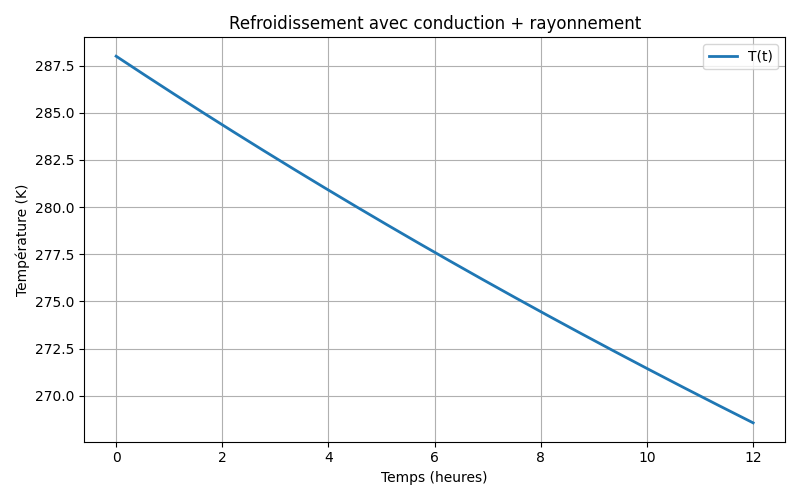
\includegraphics[width=0.8\linewidth]{../modele3/figures/modele3_coquille-conduction-rayonnement.png}    

\vspace{1cm}
\textbf{Critiques du modèle :}
\begin{itemize}
    \item Sans convection
    \item dr doit être choisi de façon à ce que la température ne varie pas significativement.
    \item Problème de définition de $T_0$ :
    \begin{itemize}
        \item température au-delà de la thermosphère (or on a posé $T_0 = 273\, \mathrm{K}$ dans nos codes Python).
    
    \end{itemize}
\end{itemize}

\newpage

\section{Modèle 4: Terre réaliste avec hétérogénéités }
\label{sec:modèle 4}
{\Large \textbf{Terre hétérogène avec rayonnement et albédo}}

\vspace{0.5cm} 
\addcontentsline{toc}{subsubsection}{Hypothèses}
\textbf{Hypothèses}


\begin{itemize}
    \item Terre modélisée avec les \textbf{continents}, les \textbf{mers}, les \textbf{océans}
    \item  On néglige: 
    \begin{itemize}
        \item convection dans l'air
        \item la conduction entre centre de la terre et croûte
        \item la conduction entre croûte et air (\(P_{th,cond}\))
    \end{itemize} 
    \item  rayonnement de la croûte (\(P_{th,ray}\))
    \item Température de l'atmosphère constante dans l'espace et au cours du temps 
    \item Prise en compte de l'albédo du sol en fonction de la position et du mois de l'année 
    \item Albédo des nuages.
    \item Capacité thermique selon la localisation
    \item $T(t=0) = T_i$ \  indépendant de l'espace  
    \item Chaleur latente considérée avec des constantes propres à chaque continent\\
    
    
    
    
\end{itemize}


\addcontentsline{toc}{subsubsection}{Schéma}

\textbf{Schéma}
\\

\noindent\textcolor{gray}{\rule{\linewidth}{0.4pt}}

    
\begin{center}
  \input{modele4/figures/Schéma modèle 4.txt }
\end{center}
\noindent\textcolor{gray}{\rule{\linewidth}{0.4pt}}
\vspace{0.5cm}
\addcontentsline{toc}{subsubsection}{Équations de transfert thermique}
\\
\textbf{Équations de transfert thermique}


On applique le premier principe appliqué au système \{ un \textbf{pavé} de la Terre, de \textbf{hauteur h} et de \textbf{surface S} \}
\ \ 
\[
\boxed{c_s \frac{dT}{dt} =(1-A_1)(1-A_2)\varphi_s-\sigma T^4+\sigma T_{atm}^4-\varphi_{lat}}
\]
Avec
\begin{itemize}
    \item \(c_s\) la capacité thermique surfacique en \(J\cdot K^{-1}\cdot m^{-2}\)
     \item  \(T\) la température du système en \(K\)
    \item \(A_1\) l'albédo des nuages (sans unité)
    \item \(A_2\) l'albédo du sol (sans unité)
    \item \(\varphi_s\) le flux solaire incident en \(W \cdot m^2\)
 \item \(\sigma\) la constante de Stefan-Boltzmann \(W \cdot m^{-2} \cdot K^{-4}\)
    \item \(T_\text{atm}\) la température de l'atmosphère en \(K\)    
    
    \item \(\varphi_{lat}\) le flux de chaleur latente émis par notre système en \(W \cdot m^2\)
\end{itemize}



\vspace{0.5cm}
\addcontentsline{toc}{subsubsection}{Tabulation de l'albédo de surface en fonction de la position :}
\\
\\
\textbf{Tabulation de l'albédo de surface en fonction de la position}

\begin{itemize}
    \item Données récupérées sur les dossiers CSV du projet (groupe B) de l'année précédente.
    \item Moyennes mensuelles tabulées pour chaque position sur Terre (latitude, longitude).
\end{itemize}
\\
\\
\addcontentsline{toc}{subsubsection}{Tabulation de l'albédo des nuages}
\textbf{Tabulation de l'albédo des nuages}

\begin{itemize}
  \item Obtenue par différence de l'albédo de la Terre lors de ciel clair et ciel nuageux (moyennes mensuelles tabulées sur 1 an, du 1er janvier 2024 au 1er janvier 2025).
\\
{Source} \href{https://ceres-tool.larc.nasa.gov/ord-tool/jsp/EBAFTOA421Selection.jsp}{ici}, code associé \href{https://github.com/pierrelouis-cmrt/CREPES/blob/main/archive/para_spaciaux/albedo/albedo_nuages_jour.py}{là}
\end{itemize}
\\
\\
\\
\\
\addcontentsline{toc}{subsubsection}{Calculs capacités calorifiques en fonction de la composition des surfaces}
\textbf{Calculs capacités calorifiques en fonction de la composition des surfaces}
\\
\\
Données récoltées \href{https://data.catds.fr/cpdc/Land_products/GRIDDED/L4SM/OPER/}{ici} et code associé \href{https://github.com/pierrelouis-cmrt/CREPES/blob/main/ressources/Cp_humidity/ZZ_cp.py}{là}.


\begin{itemize}
    \item Moyenne faite sur une période de 1 an grâce à 12 données récoltées le matin et 12 données récoltées le soir 
    \item Les 12 données ont été prises à des périodes différentes de l'année 
    \item La masse volumique de la Terre est approximée constante 
    \item Pour le \text{Groenland} et l’Antarctique  
\end{itemize}
\[
w = \frac{\rho_w \theta}{\rho_b (1 - \theta) + \rho_w \theta}
\]
Avec \(\theta\): le taux d'humidité en \(m^3\) d'eau par \(m^3\) de sol 
\[
c_p = c_{p,\text{sec}} + w (c_{p,\text{eau}} - c_{p,\text{sec}})
\]
Avec \(w\): la fraction massique d'eau 
\begin{table}[h!]
\centering
\begin{tabular}{ll}
\textbf{Constante} & \textbf{Valeur} \\
\hline
$c_{p,\text{sec}}$ & \SI{0.80}{\kilo\joule\per\kilogram\per\kelvin} \\
$c_{p,\text{eau}}$ & \SI{4.187}{\kilo\joule\per\kilogram\per\kelvin} \\
$\rho_b$ (sol) & \SI{1300}{\kilogram\per\cubic\metre} \\
$\rho_w$ (eau) & \SI{1000}{\kilogram\per\cubic\metre} \\
\end{tabular}
\caption*{Constantes utilisées pour le calcul de $c_p$}
\vspace{1cm}
\end{table}

\begin{itemize}
    \item Planisphère représentant les capacités calorifiques: 
\end{itemize}
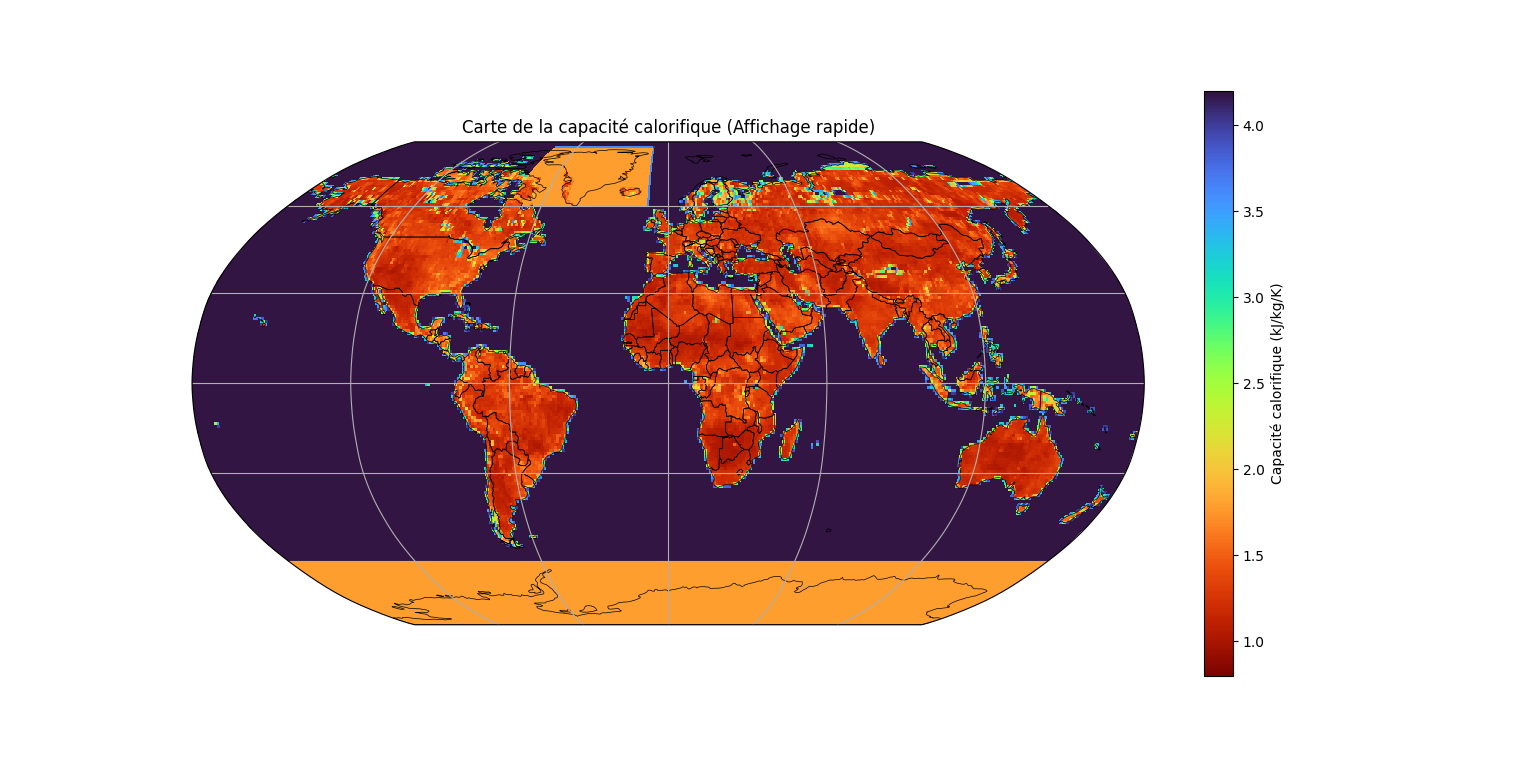
\includegraphics[width=1.0\linewidth]{modele4/figures/c_humidite.png}

\textbf{Détail du calcul de \( c_s \) :}\\
\begin{align*}
c_s &= \frac{C}{S} \\
\text{Or } S &= \frac{m}{\rho h} \\

\end{align*}

\\
\\
Avec \( C \) la capacité thermique
\\

\(h\) : profondeur à partir de laquelle la température reste constante (cf. \href{https://gitlab.com/capecl/y2/-/blob/main/Cours%20et%20exercices/Chapitre_11%20:%20Diffusion%20thermique/TD/corr_chap11_td_vprof.pdf?ref_type=heads}{exo 1, TD chap. 11 sur la diffusion thermique}), pour des variations de température journalières comprises entre 273\,K (la nuit) et 293\,K (le jour).

\\
\vspace{0.5cm}
On obtient \( h \approx 0{,}40\,\mathrm{m} \)
\\

(On nous donnait le coefficient de diffusion thermique du sol \( D_{\text{sol}} = 6 \times 10^{-7} \,\mathrm{m}^2/\mathrm{s} \))

\\
\vspace{0,5cm}
\\

\addcontentsline{toc}{subsubsection}{Chaleur latente}
\textbf{Chaleur latente}
\\


$\rightarrow$ correspond à la puissance surfacique positive (reçue) ou négative (fournie) afin d'évaporer ou de condenser l'eau de la surface de la Terre.\\

$\rightarrow$ On découpe la Terre de plusieurs manières, par mers et océans, et par continents.\\[0.5em]


\\
On parle d'une moyenne faite par continents :

\begin{itemize}
    \item Mers et océans : 108.8 $W/m^2$
    \item Asie : 28.8 $W/m^2$
    \item Afrique : 45.1 $W/m^2$
    \item Europe : 38.1 $W/m^2$
    \item Amérique du Nord : 36.5 $W/m^2$
    \item Amérique du Sud : 73.1 $W/m^2$
    \item Océanie : 31.9 $W/m^2$
\end{itemize}

On suppose que la pression atmosphérique de la Terre est constante à la surface. 

\vspace{0.5cm}
On applique le premier principe de la thermodynamique :

\vspace{0.5cm}
\begin{align*}
    dH &= \delta Q \\
    dm \, \Delta h_{\text{vap}} &= P_{th} \times dt \\
    Dm \, \Delta h_{\text{vap}} &= P_{th}
\end{align*}

Donc, 
\begin{align*}
    \phi_{\text{lat}} &= \frac{Dm}{S} \Delta h_{\text{vap}} \\
    \phi_{\text{lat}} &= \frac{m}{S \Delta t} \Delta h_{\text{vap}} \\
    \phi_{\text{lat}} &= \frac{\rho V}{S \Delta t} \Delta h_{\text{vap}} \\
    \phi_{\text{lat}} &= \boxed{\frac{\rho S E_{\text{vap}} \Delta t}{S \Delta t} \Delta h_{\text{vap}}}
\end{align*}






Avec \( E_{\mathrm{vap}} \) l'\href{https://environmentofearth.wordpress.com/2008/03/11/water-balance/?}{évaporation} en m/s.


\\

\begin{tabular}{|c|c|}
\hline
Continents & évaporation ($\mathrm{cm/year}$) \\
\hline
Europe & 49 \\
\hline
Amérique du Nord & 47 \\
\hline
Amérique du Sud & 94 \\
\hline
Afrique & 58 \\
\hline
Asie & 37 \\
\hline
Océanie & 41 \\
\hline
Océans & 140 \\
\hline
\end{tabular}
\\

\\
On obtient donc:

\\
\vspace{0,5cm}
\\
\begin{tabular}{|c|c|}
\hline
Continents & Flux de chaleur latente ($\mathrm{W/m^2}$) \\
\hline
Europe & 38.1 \\
\hline
Amérique du Nord & 36.5 \\
\hline
Amérique du Sud & 73.1 \\
\hline
Afrique & 45.1 \\
\hline
Asie & 28.8 \\
\hline
Océanie & 31.9 \\
\hline
Océans & 108.8 \\
\hline
\end{tabular}
\\
\\
\addcontentsline{toc}{subsubsection}{Modélisation graphique}

\textbf{Modélisation graphique : }
\\
\\
Commentaire général: 
\begin{itemize}
    \item La deuxième année est simulée afin de laisser le temps à la température de se stabiliser, car des artefacts apparaissent au début de la première année (T initiale fixée à 15 °C)
    \item Un lissage par convolution gaussienne est appliqué aux grandeurs tabulées (albédo de surface et des nuages, chaleur latente) pour atténuer les discontinuités liées aux transitions jour/nuit et aux changements mensuels
    \item \href{https://github.com/pierrelouis-cmrt/CREPES/blob/main/modele4/code/modele_courbe.py}{code des premiers graphiques}
\end{itemize}


\begin{center}
  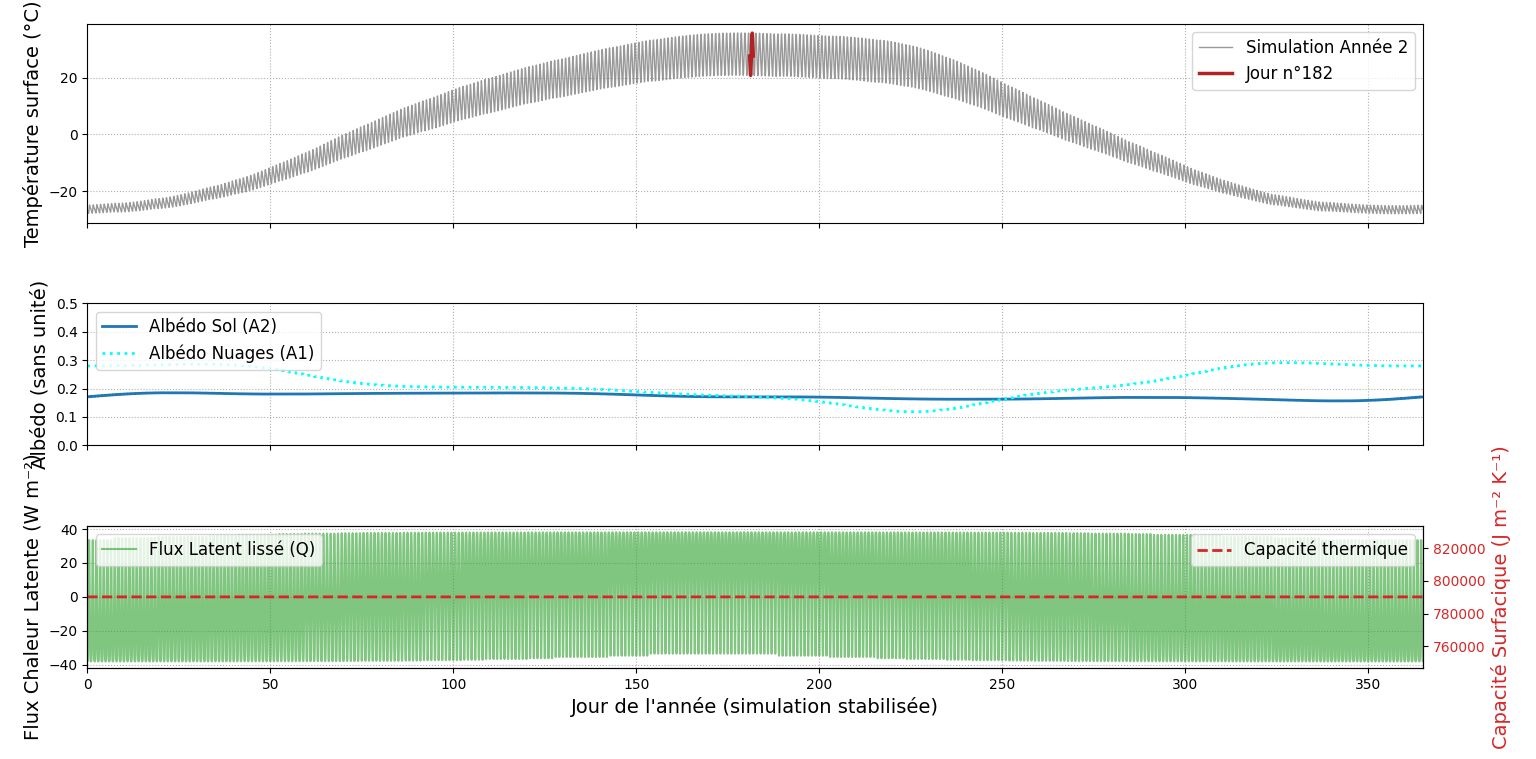
\includegraphics[width=1\linewidth]{modele4/figures/paris.png}
  \textbf{Figure :} Simulation de l'évolution de la température sur une année à \textbf{Paris}
\end{center}
\textbf{Paris :}
\begin{itemize}
    \item 	La légère montée du min et du max de la chaleur latente après lissage vient  du fait que la durée du jour varie au fil de l’année 
    \item Les variations journalières sont un peu trop faibles en hiver
    \item La température globale est trop basse
\end{itemize}

  
\begin{center}
  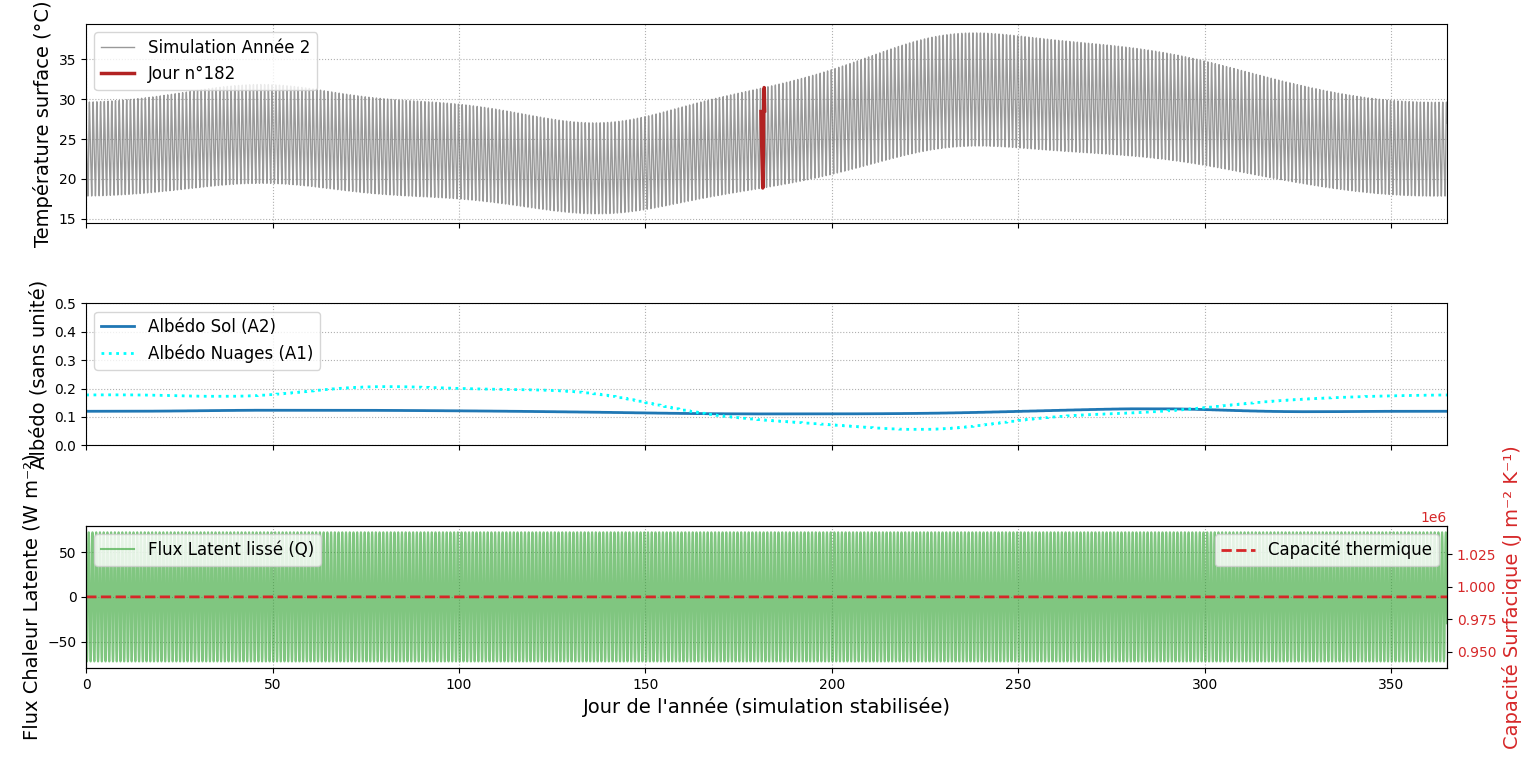
\includegraphics[width=1\linewidth]{modele4/figures/amzonie.png}
  \textbf{Figure :} Simulation de l'évolution de la température sur une année en Amazonie
  \end{center}
  \textbf{Amazonie}
\begin{itemize}
    \item La température globale évolue de manière cohérente avec le cycle saisonnier : elle diminue pendant la saison des pluies et augmente pendant la saison sèche.
    \item L’albédo des nuages suit également ces variations, avec une évolution logique selon les saisons.
\end{itemize}

\\

\\
  
\begin{center}
  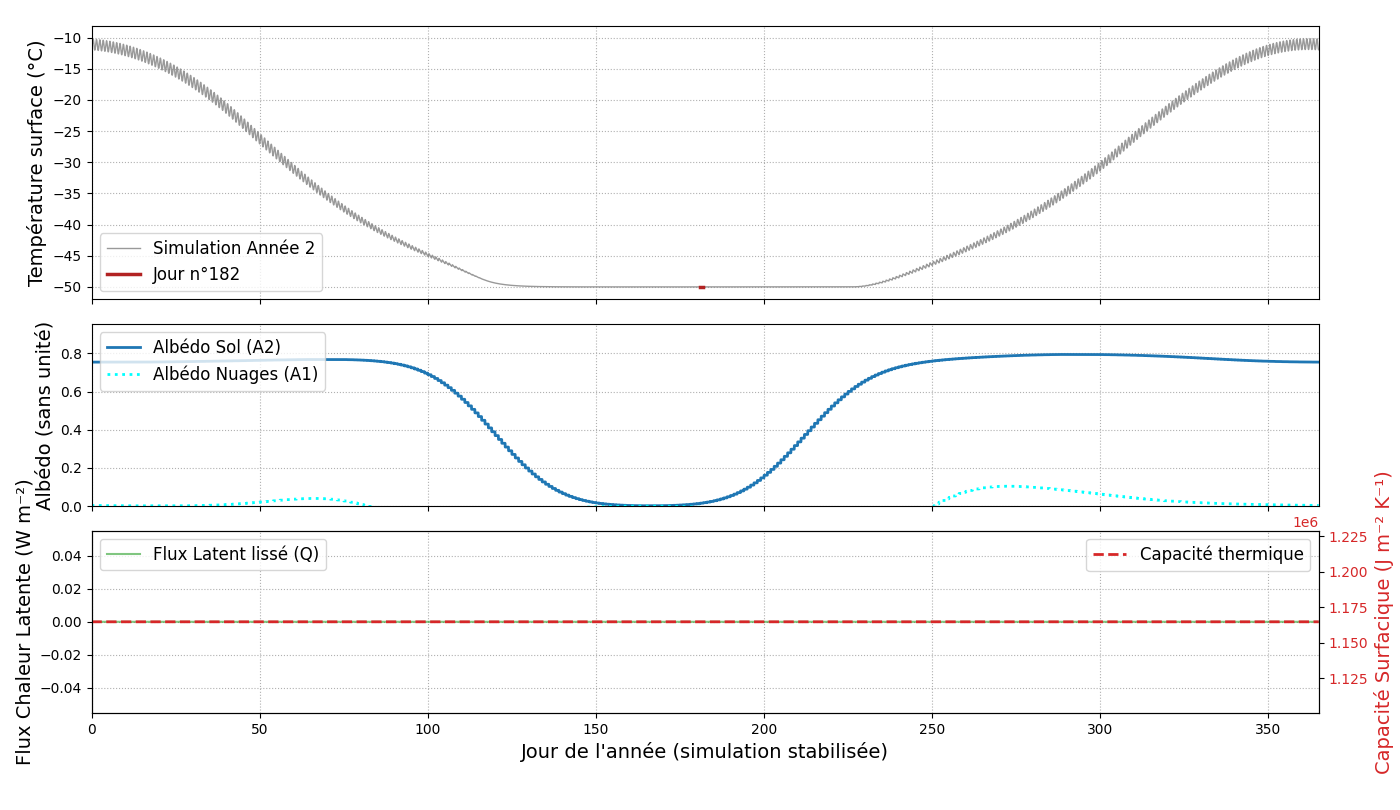
\includegraphics[width=1\linewidth]{modele4/figures/antarctique.png}
  \textbf{Figure :} Simulation de l'évolution de la température sur une année en Antarctique
  \end{center}
\textbf{ Antarctique}
\begin{itemize}
    \item La température globale simulée est trop élevée par rapport aux valeurs attendues.
    \item La courbe de température est artificiellement aplatie en milieu de période car la température atmosphérique (\texttt{Tatm}) est fixée à $-50\,^\circ$C, ce qui empêche la température de descendre en dessous.
    \item Il existe une période où l’albédo du sol est nul, car la valeur tabulée dans le fichier CSV ($\sim 0{,}0001$) est arrondie à zéro dans les calculs.
\end{itemize}

  \begin{center}
  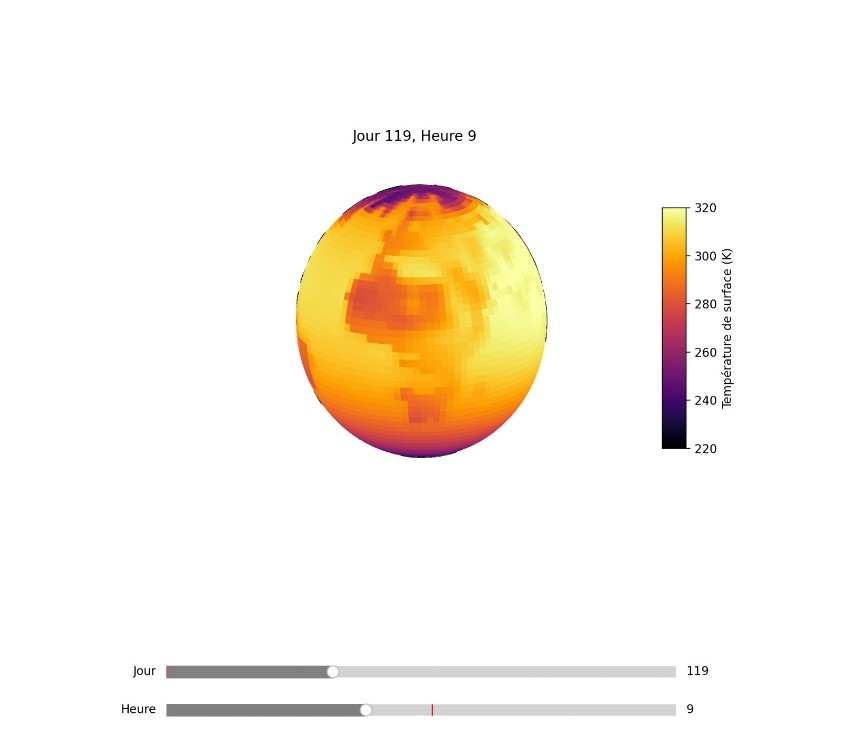
\includegraphics[width=1\linewidth]{modele4/figures/plan1.jpg}
  
  \end{center}

\href{https://github.com/pierrelouis-cmrt/CREPES/blob/main/modele4/code/modele_sphere_haute_res.py}{Code associé}  

  \begin{center}
  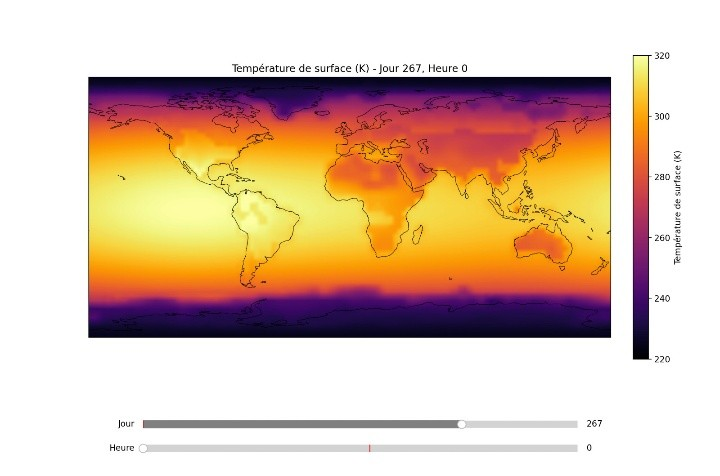
\includegraphics[width=1\linewidth]{modele4/figures/plan2}
  
  \end{center}
  \\ 
\href{https://github.com/pierrelouis-cmrt/CREPES/blob/main/modele4/code/modele_planisphere_haute_res.py}{Code associé}


\\
\vspace{0,5cm}
\\

\addcontentsline{toc}{subsubsection}{Critique du modèle}
\textbf{Critique du modèle}

\begin{itemize}
    \item On néglige la conducto-convexion
    \item température de l'atmosphère considérée homogène et constante au cours du temps
    \item Les valeurs de chaleur latente sont prises constantes, ce qui n'est pas le cas en réalité
\end{itemize}
\end{document}